\documentclass{article}
\usepackage[margin=0.625in]{geometry}
\usepackage{parskip, setspace}
\setstretch{1.15}
\usepackage{amsmath, amsfonts}
%\numberwithin{equation}{subsection}
\usepackage{graphicx, caption}
\usepackage{hyperref}
\usepackage[ruled, linesnumbered, noend]{algorithm2e}

\title{CS 529: Advanced Data Structures \& Algorithms \\ Assignment 1}
\author{Nathan Chapman, Hunter L., Andrew Struthers}
\date{\today}

\begin{document}
\maketitle

\section*{Creating a 3-2 Tree}



    \begin{function}
        \caption{bumpAndBreak(p)}
        \DontPrintSemicolon

        \KwIn{node $p$}
        \KwOut{Null}

        \eIf{p has a parent}{
            insert $p.keys[2]$ into $p.parent.keys$
        }{
            create parent node with key $p.keys[2]$\;
        }
        remove $p.keys[2]$\;
        create $parent.left$ with key $min \ p.keys$\;
        create $parent.right$ with key $max \ p.keys$\;
        remove $parent.middle$\;
    \end{function}

    \begin{function}
        \caption{insertRecursive(p, k)}
        \DontPrintSemicolon

        \KwIn{node $p$, new key $k$}
        \KwOut{3-2 B-tree}

        \If{$p$ is a leaf}{
            insert $k$ into $p.keys$\;
            sort $p.keys$\;
            \If{length of p.keys = 3}{
                bumpAndBreak(p)
            }
        }
        \ElseIf{$k < p.keys[1]$}{
            \insertRecursive(p.left, k)\;
        }
        \ElseIf{$k > p.keys[end]$}{
            \insertRecursive(p.right, k)\;
        }
        \Else{
            \insertRecursive(p.middle, k)\;
        }
    \end{function}

    \begin{function}
        \caption{buildTree(keyList)}
        \DontPrintSemicolon

        \KwIn{List of keys}
        \KwOut{3-2 Tree of given keys}

        create root node with key $keyList[1]$\;

        \ForEach{$key \in keyList[2:end]$}{
            insertRecursive(root, key)
        }
    \end{function}

\pagebreak

\section*{Discussion on van Emde Boas Trees}

van Emde Boas (vEB) trees store a fixed number of n bits in an index-addressable structure, the length of which must be an order of $2m$. Each bit position represents the presence of that value in that structure. From this list, it constructs a summary vector tree storing binary values identifying the presence of a positive bit within its vector. An example of a vEB tree of order $16$ can be seen below.

\begin{figure}[h]
    \centering
    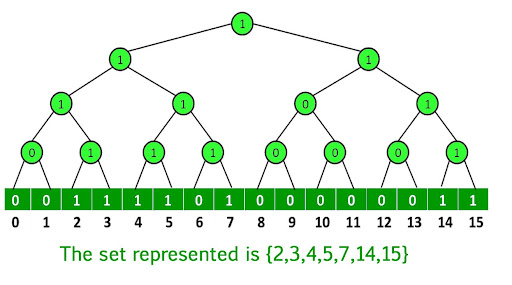
\includegraphics[scale=0.5,keepaspectratio]{Images/vebtree.jpg}
    \label{fig:veb_tree}
    \caption{Van Emde Boas Trees (``proto van Emde Boas Trees". geeksforgeeks.org)}
\end{figure}

Unlike other structures, the index addressable structure it is built on allows for insertion, deletion, and searching in constant $O(1)$ time simply by changing the bit at the index representing the value in the tree and updating the summary vector. The major strength of vEB trees is in its ability to find the next nearest value from any given value in $O(\text{log}\text{log} M)$ time ($M$ being the total number of possible integers in $2m$).

An example use case for vEB trees may be in the location of the nearest empty parking space. Assuming that the car is near a parking space, that the spaces are ordered by distance from one another (i.e. space \#3 is closer to space \#5 than space \#10), and that a $1$ represents an empty parking space. After locating the current spot in constant time (which we will assume to be full), the ability of vEB trees to find a successor (or predecessor) of an empty spot in $O(\text{log}\text{log} M)$ might prove useful.

Unfortunately, the limitations of vEB trees make other algorithms (such as Skip Lists) much more preferable for solving successor and predecessor problems. While the constant time insertion and deletion are ideal, the limitation that they may only represent integers values is a major limitation. The fixed size also restricts what the structure can represent. And finally, the fixed space requirement of $O(M)$ makes the structure cumbersome. These drawbacks, combined with the fact that structures like Skip Lists can perform next nearest neighbor functions on more versatile objects in $O(\text{log} n)$ time, makes them more useful over vEB trees.

\pagebreak

\section*{Discussion on Skip Lists}

Skip lists are an extension on the standard linked list. This data structure on average preserves the space efficiency of a linked list, but due to the random nature of this structure, could have worst case $O(n \text{log} n)$ space efficiency. Skip lists also have the insertion/deletion ease of a linked list, where each node in the list has a pointer to the next (and sometimes previous) node, while also benefiting from the searching speed of various tree structures. This data structure is a randomized data structure, and it allows an average complexity of $O(\text{log} n)$ for insertion and searching. This means that on average, a skip list has the best features of a sorted array, capable of random memory access while searching, while maintaining the linked list structure, meaning that insertion requires very low time complexity. 

A skip list can be thought of as a layered linked list. The bottom layer is denoted as $L(0)$, and then higher layers are denoted as $L(1)$, $L(2)$, \ldots, $L(n)$. An element of the skip list has a $\frac{1}{2^m}$\% chance of being on layer m. If an element appears on layer m, the element also must appear on layer $m-1$, $m-2$, \ldots, $0$. An image of a skip list can be seen below

\begin{figure}[h]
    \centering
    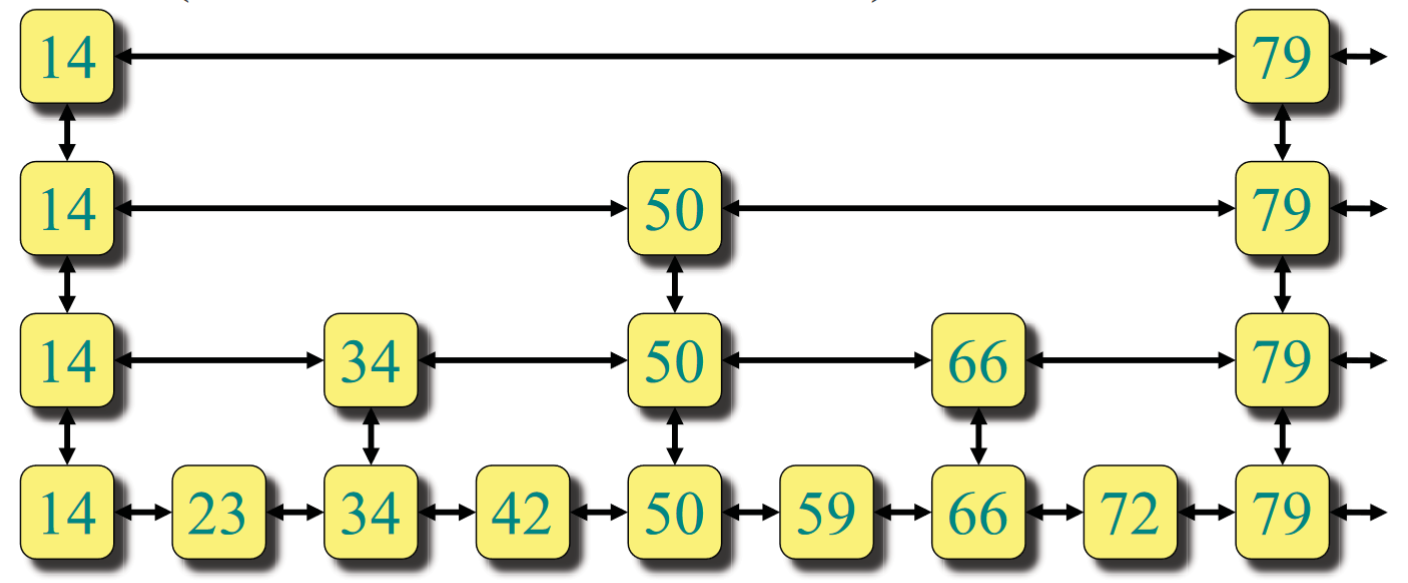
\includegraphics[width=\textwidth,keepaspectratio]{Images/SkipList_MIT.PNG}
    \label{fig:skip_list}
    \caption{An example of a skip list from the MIT lecture slides}
\end{figure}

The hierarchical structure of the layers results in an average time complexity of $O(\text{log} n)$ for search, insert, and delete operations and a worst case of $O(n)$. This structure uses randomness and a layered linked list to skip over portions of the data when performing search operations, to a very similar effect as a binary search tree. The linked list structure is more beneficial than a binary search tree, however, because there is no need to rebalance the tree after every insertion or deletion with a skip list.

A common real-world representation of a skip list is buses in a busy city. In downtown Seattle, for example, there are many bus stops. Some buses go from stop to stop, whereas some buses stop at one high traffic stop, then cross town, skipping many lower traffic stops in the process. This is the same idea as a skip list, where the bottom row is analogous to the bus that stops at every destination, and the higher up rows in the skip list hierarchy are analogous to the buses that take people from one high traffic destination to another, skipping over some stops. 

Skip lists have many applications, especially in high traffic operations where rebalancing a tree or linearly searching through a massive array would take too long. One of the common applications of skip lists in industry is using this data structure as a way to index databases and database tables. Another application of skip lists is in priority queues, where one specific example could be CPU job scheduling. CPU job scheduling is a very time-sensitive process, where jobs could be swapped out many times per second. Maintaining a priority queue with a skip list, where each node in the list is a priority of a job, allows the priority queue to operate in logarithmic time, where insertion and deletion is much faster than a standard queue implementation, and a tree structure doesn’t need to be constantly maintained and rebalanced as jobs get added to or removed from the system.



\pagebreak

\end{document}